\section{Setting up the Workspace for C Projects}

\textbf{Objectives for this tutorial:}
\begin{itemize}
	\item create all needed library projects (runtime.c and modellib.c)
	\item create the tutorial project with the examples
	\item create the project with a traffic light simulator
	\item test the workspace setup by running one of the examples
\end{itemize}

\subsection{Create Library, Tutorial and Simulator Projects}

Before you can start with C, some preconditions must be fulfilled:

\begin{itemize}
\item A C compiler must be installed on your machine. All tutorials are based on MinGW/GCC (Windows) and Posix/GCC (Linux), but currently only tested on Windows with MinGW/GCC
\item The CDT-Eclipse plugin must be installed as the C development environment.
\end{itemize}

After installation of eclipse and the \eTrice{} plug in, your workspace should look like this:  

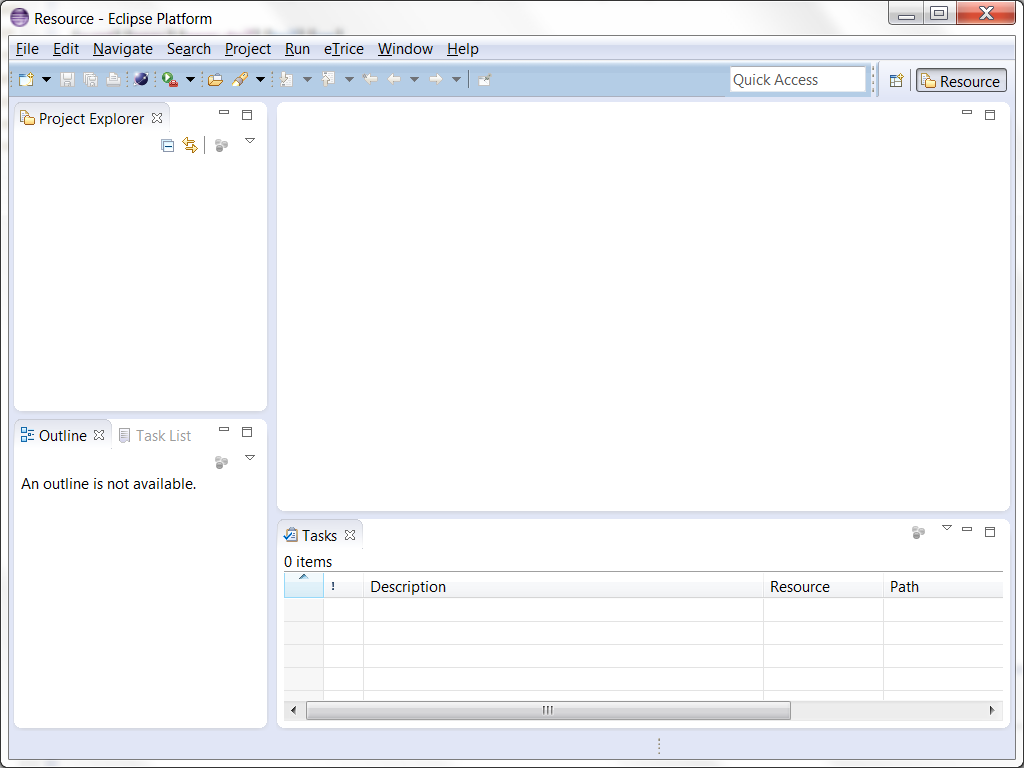
\includegraphics[width=0.8\textwidth]{images/013-SetupWorkspace01.png}
% !images/013-SetupWorkspace01.png!

Just the \eTrice{} menu item is visible of the installed \eTrice{} plugins.

\newpage
Select the menu \emph{File->New->Other}

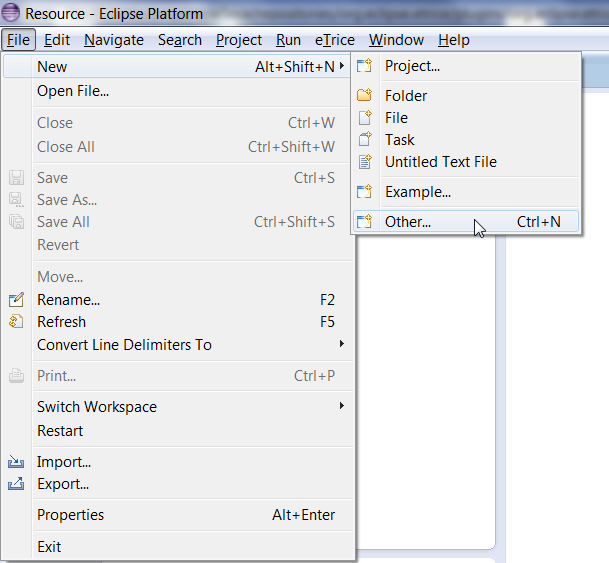
\includegraphics[width=0.6\textwidth]{images/013-SetupWorkspace02.png}
% !images/013-SetupWorkspace02.png!

Open the \emph{eTrice} tab and select \textit{eTrice C Runtime}

Press \emph{Next} and \emph{Finish} to install the Runtime into your workspace.

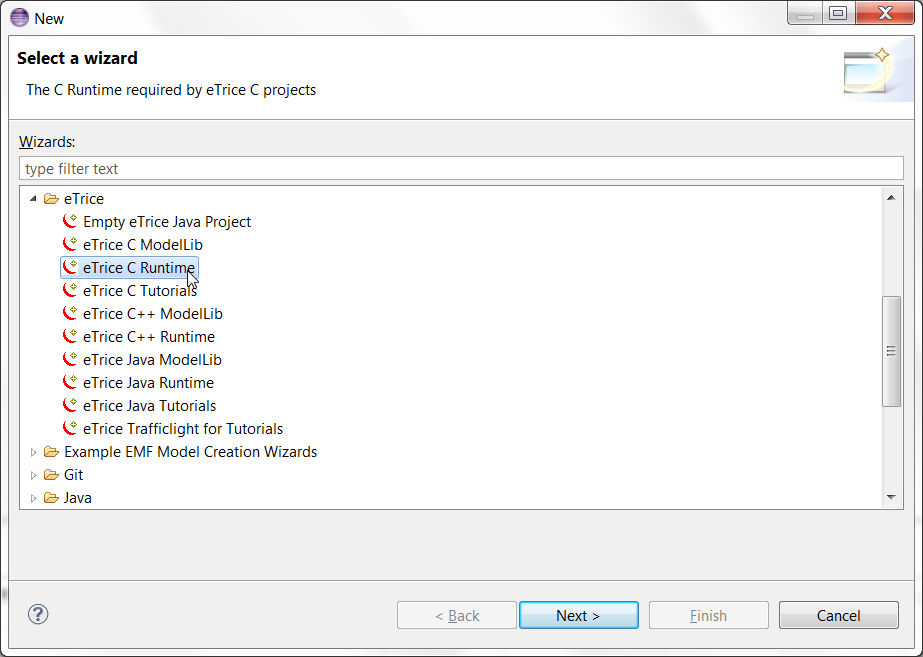
\includegraphics[width=0.6\textwidth]{images/014-SetupWorkspaceC005.png}
% !images/014-SetupWorkspaceC005.png!

\newpage
Do the same steps for \textit{eTrice C Modellib}, \textit{eTrice C Tutorials} and \textit{eTrice Trafficlight for Tutorials}. To avoid temporary 
error markers you should keep the proposed order of installation. The resulting workspace should look like 
this:

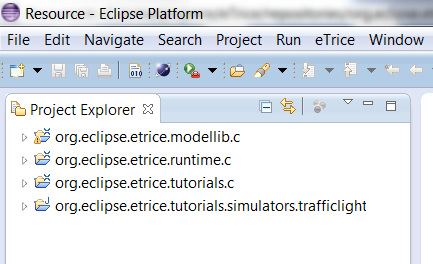
\includegraphics[width=0.5\textwidth]{images/014-SetupWorkspace007.png}
% !images/014-SetupWorkspace007.png!

\subsection{Perform Setup Test}

To check the correct setup of your workspace we run a little testproject contained in the tutorial project.

The tutorial models are available in the  \emph{org.eclipse.etrice.tutorials.c} project. All tutorials are ready to generate and run without any changes. To test the code generator and the workspace setup simply run 
\emph{gen\_SetupTestC.launch} as \emph{gen\_SetupTestC}: 

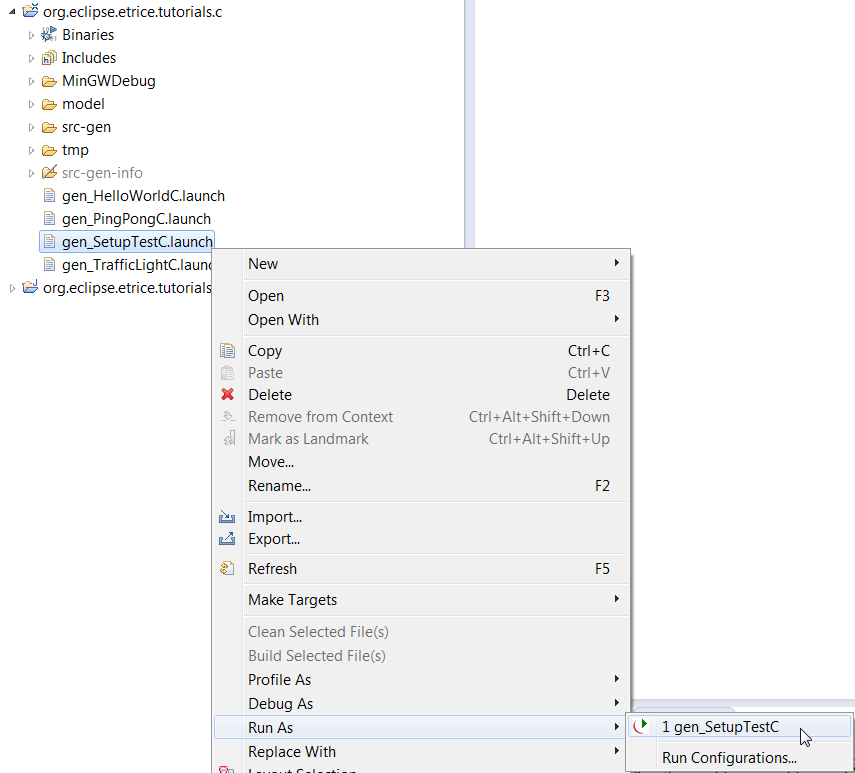
\includegraphics[width=0.6\textwidth]{images/014-05-gen_SetupTestC.png}
% !images/014-05-gen_SetupTestC.png!

\newpage
The successful generation ends with \emph{Info: -- finished code generation} in the Console.

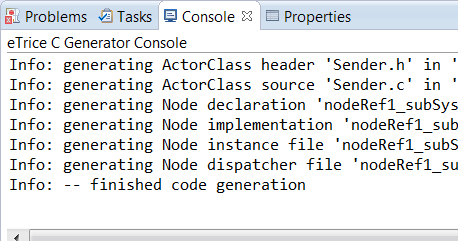
\includegraphics[width=0.5\textwidth]{images/014-06-FinishedCodeGeneration.png}
% !014-06-FinishedCodeGeneration.png!

For each tutorial in the folder src-gen a sub folder is generated which contains the generated code. The file \emph{<...>\_Runner.c} contains the main function. To run the generated application you first have to compile the project (with the hammer symbol in the C/C++ Perspective).

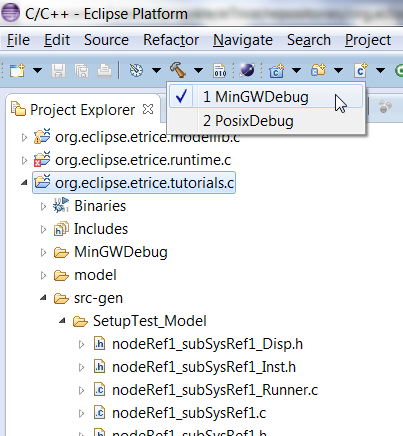
\includegraphics[width=0.5\textwidth]{images/014-07-Compile.png}
% !014-07-Compile.png!

If the compilitation does not succeed, make sure to clean and compile the projects \emph{org.eclipse.etrice.runtime.c} and \emph{org.eclipse.etrice.modellib.c} with the correct build configuration for your platform. Depending on the setup of your C compiler and CDT you might have to change the pre defined build configurations \emph{MinGWDebug} or \emph{PosixDebug}.

After the successful compilation you can run the application as \emph{Local C/C++ Application}.

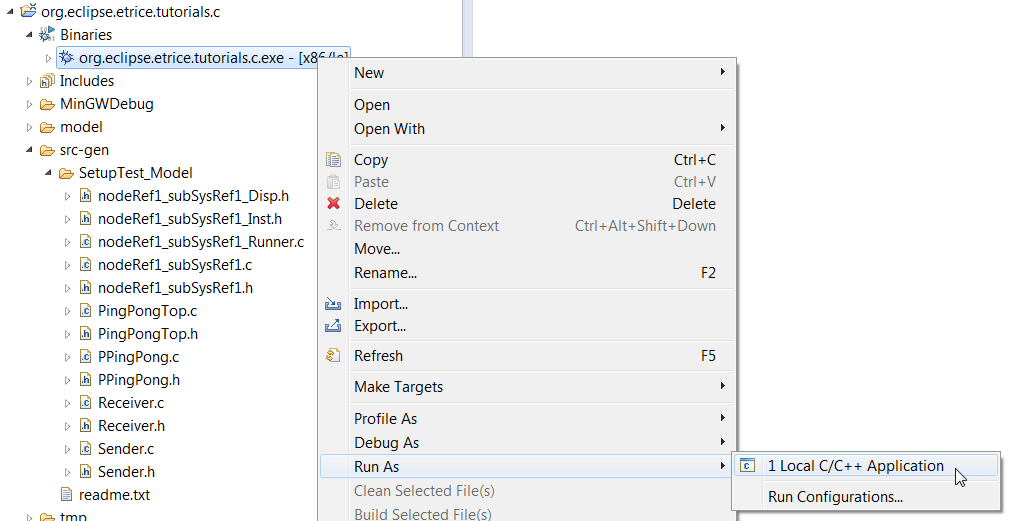
\includegraphics[width=0.7\textwidth]{images/014-08-RunAsC-CPP-Application.png}
% !images/014-08-RunAsC-CPP-Application.png!

\newpage
To stop the application type \emph{quit} in the console window. If your Console contains the lines
\newline\emph{******************}
\newline\emph{*** Setup OK ***}
\newline\emph{******************} 
\newline your setup should be ok.

%TODO : update screenshot
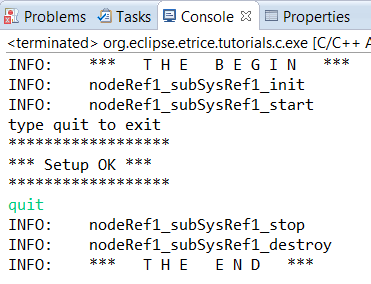
\includegraphics[width=0.6\textwidth]{images/014-09-ConsoleWithSetupOk.png} 
% !images/014-09-ConsoleWithSetupOk.png!

Now the workspace is set up and you can perform the tutorials or start with your work.

